\subsection*{Phylogenetic Structure and association with host data}
\graphicspath{{images/phylogeneticStructureHostData/}}


% Phylogenetic analysis and association with host data: comparison of phylogenetic
% trees based on accessory gene presence/absence or on core gene alignment.
% Do you detect clusters of strains? How do they associate with the metadata?

A significant difference is found between the tree obtained from the presence/absence of genes
and the one built from the core gene alignement (figure \ref{fig:phylogenetic trees}). Instead,
MAFFT and PRANK produced core gene alignements that resulted in identical trees (figure \ref{core alignement mafft tree}).

Three clusters were seen in every tree, but the low number of samples and the high fragmentation of
information seen in the metadata impede the observation of finer clustering. The sample 
classified as \emph{non-westernized} always clustered alone in the trees.


\begin{figure}[h!]
    \centering
    \begin{subfigure}[b]{0.7\textwidth}
        \centering
        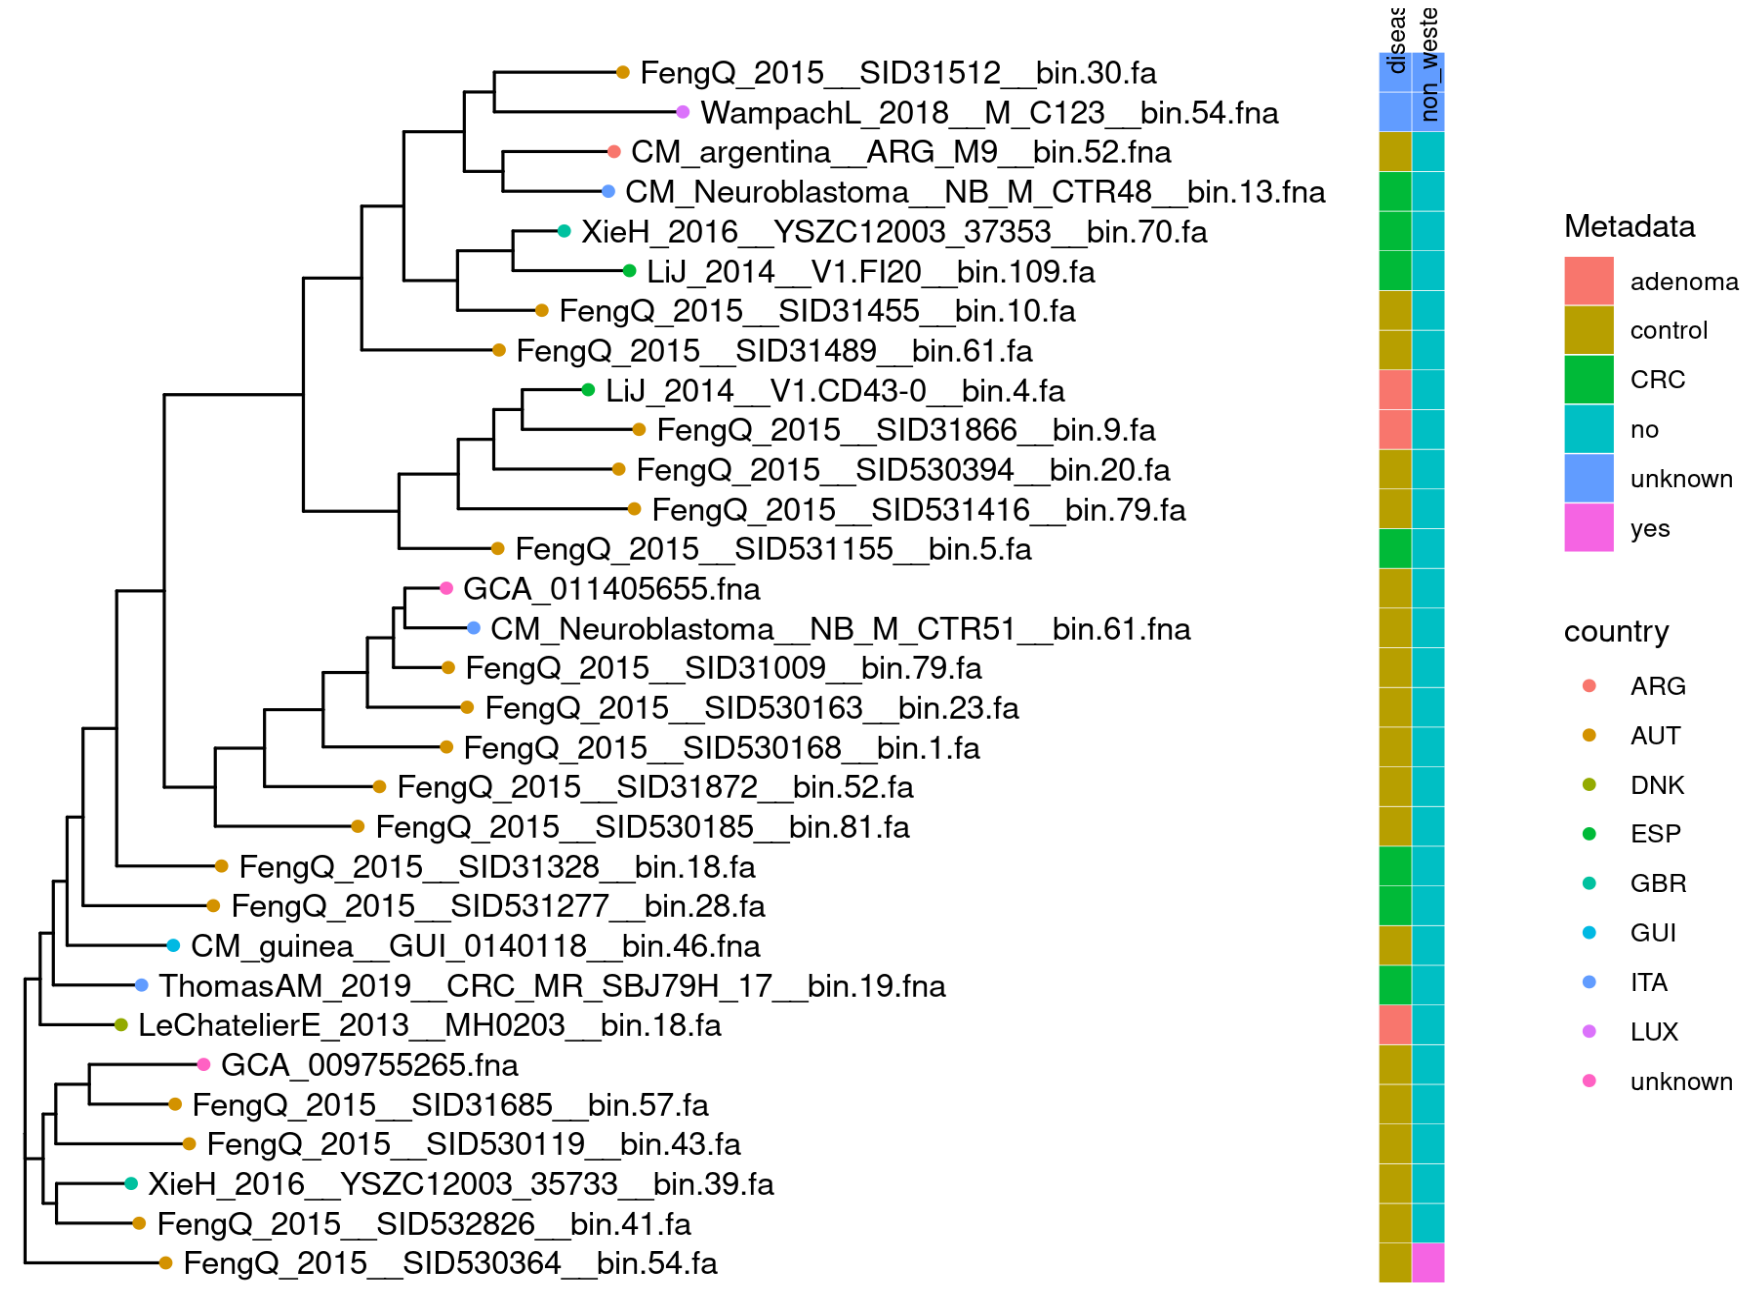
\includegraphics[width=\textwidth]{enriched_tree.png}
        \caption{}
        \label{fig:core alignment prank tree}
    \end{subfigure}
    \begin{subfigure}[b]{0.7\textwidth}
        \centering
        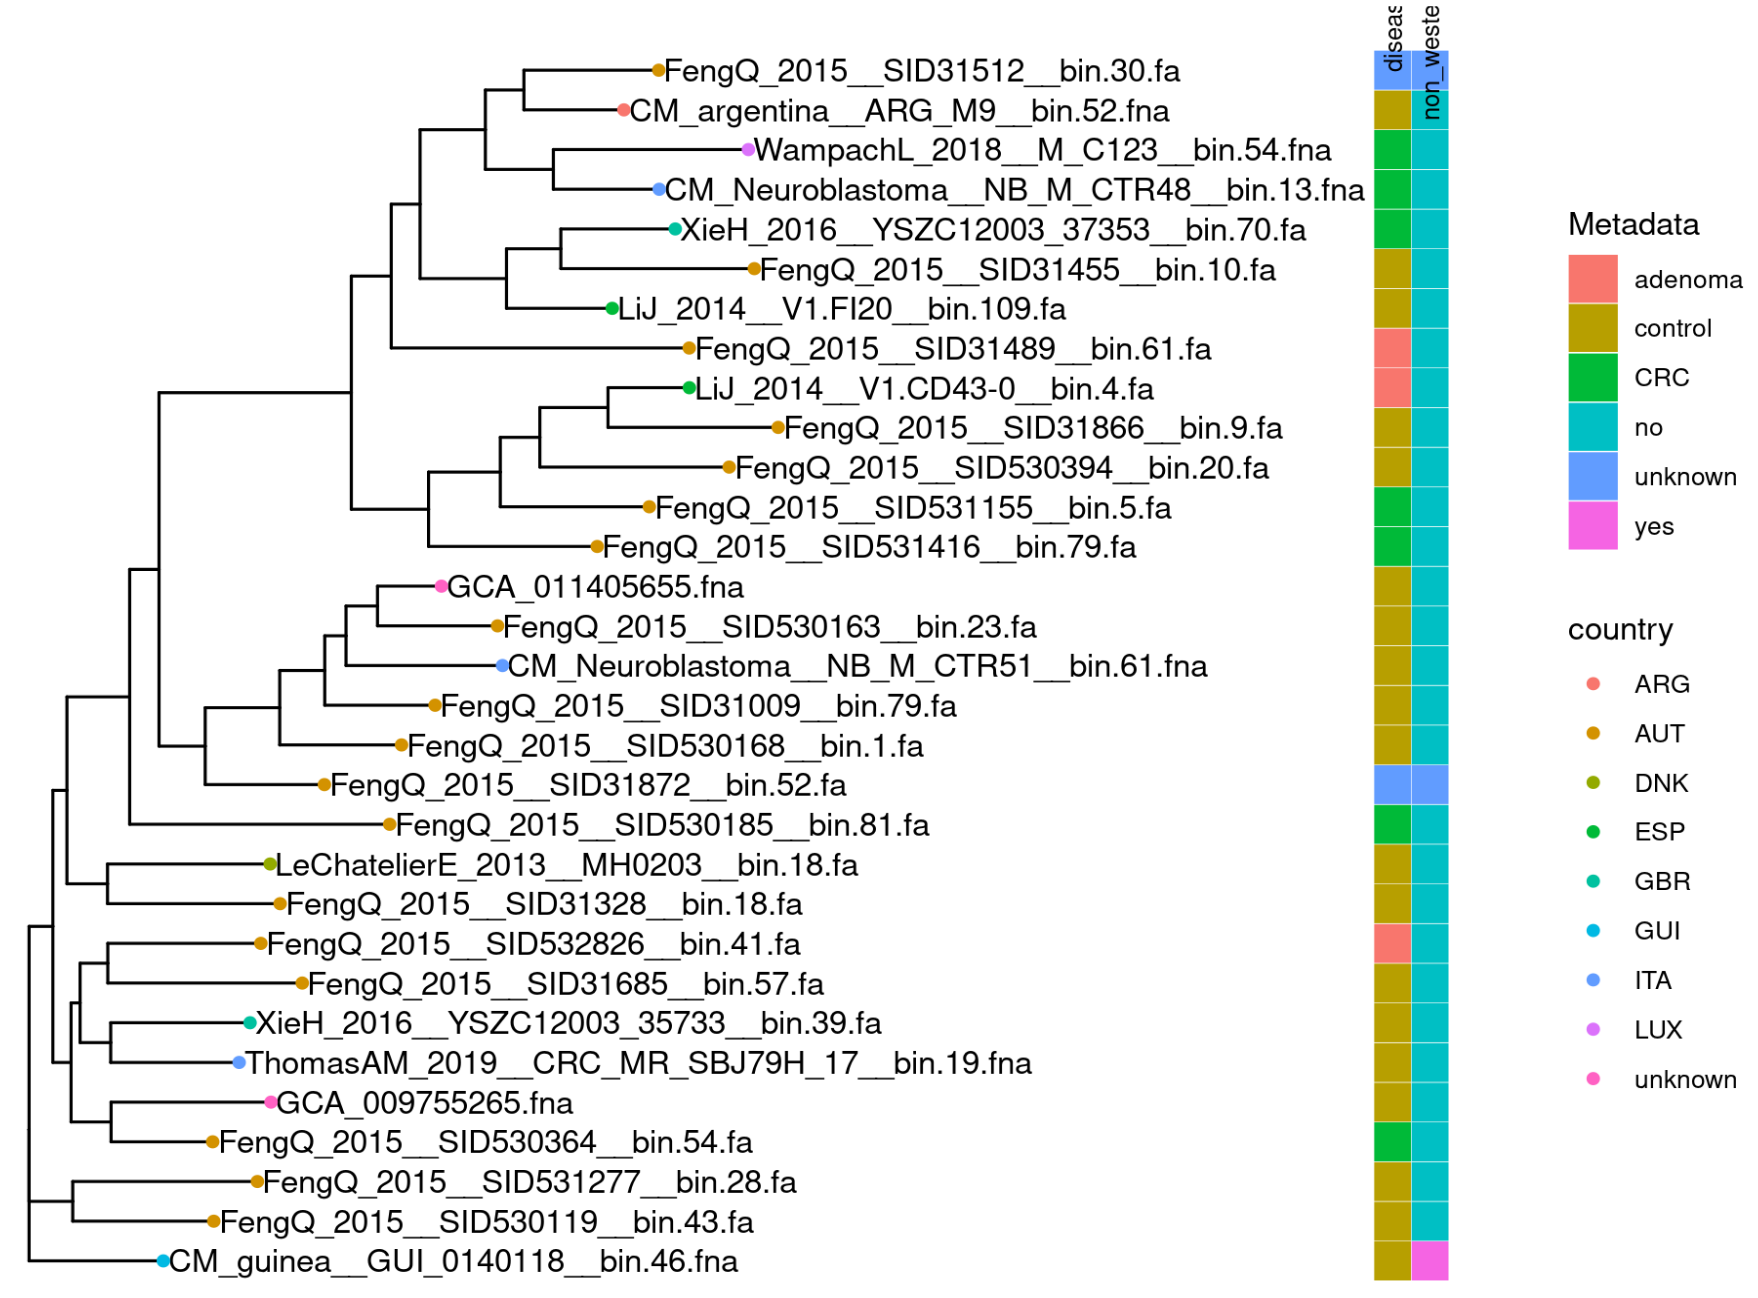
\includegraphics[width=\textwidth]{enriched_tree_newick.png}
        \caption{}
        \label{fig:presence absence tree}
    \end{subfigure}
       \caption{}
       \label{fig:phylogenetic trees}
\end{figure}


